% Follow-on paper to:
%   Holmes, S. A. "Cryptographic Authentication for Private RAG-Enabled
%   LLMs."  AISecPriv 2025.
%
% Self-contained — compiles with pdflatex + bibtex.

\documentclass[11pt,a4paper]{article}

\usepackage[utf8]{inputenc}
\usepackage[T1]{fontenc}
\usepackage[margin=1in]{geometry}
\usepackage{microtype}
\usepackage{booktabs}
\usepackage{multirow}
\usepackage{siunitx}
\sisetup{
  group-separator      = {,},
  group-minimum-digits = 4,
  detect-weight        = true,
  detect-family        = true,
}
\usepackage{amsmath}
\usepackage{amssymb}
\usepackage{amsthm}
\usepackage{xcolor}
\usepackage{listings}
\usepackage{hyperref}
\usepackage{url}
\usepackage{tikz}
\usepackage{pgfplots}
\pgfplotsset{compat=1.18}
\usepackage{algorithm}
\usepackage{algpseudocode}

\hypersetup{
  colorlinks   = true,
  linkcolor    = blue!50!black,
  citecolor    = blue!50!black,
  urlcolor     = blue!50!black,
}

\newtheorem{theorem}{Theorem}
\newtheorem{definition}{Definition}
\newtheorem{property}{Property}

\title{
  Layered Drift Defence and AI-Safety Gating \\
  for RAG-Authenticated LLMs
}
\author{Stephen A. Holmes \\
  University of Surrey \\
  \texttt{s.a.holmes@surrey.ac.uk}}
\date{2026}

\begin{document}

\maketitle

\begin{abstract}
The RAG\nobreakdash-Sign scheme of \cite{holmes2025ragsign} binds the
signing key of a Retrieval\nobreakdash-Augmented Generation system
to a tuple of $(\mathit{model\_hash}, \mathit{lsh\_key},
\mathit{hsm\_secret})$ via a fuzzy extractor over a MinHash sketch
of the corpus.  We extend the construction in four directions and
report empirical results from a 3{,}000\nobreakdash-line open\nobreakdash-source
reference implementation.  First, we reproduce the paper's
\SI{5}{\percent} drift threshold on the actual IACR ePrint Archive
corpus (\num{12036} papers, \SI{966}{\mega\byte}) and find it
holds with 16 bits of headroom against a $T = 30$ BCH bound; the
empirical failure cliff lies at $\sim\!\SI{12}{\percent}$ corpus drift.
Second, we factor the single threshold of the original paper into a
\emph{layered} model with two distinct ceilings — the cryptographic
BCH bound and a configurable operator policy — and add
\textsf{check\_drift} / \textsf{regenerate} primitives for clean
key rotation when the policy fires.  Third, we add an external
\emph{regulator authority} with two operations: signed
\textsf{ROTATE} / \textsf{REVOKE} directives that the deployment
verifies against a registered ECDSA public key, and a secure\nobreakdash-sketch
audit primitive that lets the regulator verify corpus integrity
remotely without seeing corpus content.  Fourth, we attempt to lift
the drift\nobreakdash-tolerant pattern to the \emph{model} layer for
AI\nobreakdash-safety gating, and find that the natural weight\nobreakdash-space
SimHash is empirically too conservative — even a 1{,}000\nobreakdash-step
fine\nobreakdash-tune of GPT\nobreakdash-2 small flips only $3$ of
$512$ bits.  We therefore introduce a \emph{behavioural} fingerprint
that hashes the model's outputs on a fixed probe set instead of its
weights, and show this is ${\sim}\!9$\textendash$13\!\times$ more
sensitive at the same fine\nobreakdash-tune intensity, giving the
AI\nobreakdash-safety gate a usable operating curve.  Finally, we
formulate and run a multi\nobreakdash-seed test of a
\emph{differential\nobreakdash-drift conjecture}
(Section~\ref{sec:poisoning}): that for fixed fine\nobreakdash-tune
budgets, fingerprint drift on contradictory training data should
exceed drift on coherent training data because contradictory data
forces the optimiser to unlearn before re\nobreakdash-learning.  We
find a striking \emph{regime\nobreakdash-dependent} signal: at
$5$ SGD steps contradictory data drifts $1.82\!\times$ more than
coherent ($3$\nobreakdash-of\nobreakdash-$3$ seeds, mean $13.3$ vs.\
$7.3$ bits), but by $25$ steps the differential collapses or
reverses as the optimiser memorises the small contradictory
corpus.  The signal lives in the early\nobreakdash-training
\emph{trajectory}, not in the final fingerprint — a
deployment\nobreakdash-relevant finding because it suggests
sampling the fingerprint mid\nobreakdash-training rather than
post\nobreakdash-training.  All numbers are reproducible from the
open\nobreakdash-source reference
implementation~\cite{ragsign-impl}.  All numbers are reproducible
from the open\nobreakdash-source reference
implementation~\cite{ragsign-impl}.
\end{abstract}

\section{Introduction}
\label{sec:intro}

The RAG\nobreakdash-Sign construction \cite{holmes2025ragsign} solves a
specific and increasingly\nobreakdash-pressing problem in the deployment of
generative AI: \emph{provenance binding for retrieval\nobreakdash-augmented
generation}.  The deployment runs an LLM (the paper specifies
\texttt{Llama 3.2 2B}~\cite{llama-cpp-python}) over a private
corpus (the paper proposes the IACR ePrint Archive) and a hardware\nobreakdash-protected
secret.  Algorithm~1 of the paper binds these into a deterministic
ECDSA signing key whose public half becomes the deployment's
long\nobreakdash-term identity.  Outputs are signed; the public key on the
allow\nobreakdash-list both authorises queries and acts as a global
kill\nobreakdash-switch when revoked.

Real deployments have to reckon with three operational concerns the
original paper acknowledges but does not fully address:

\begin{enumerate}
  \item \textbf{Two thresholds, not one.}  §6.5 specifies a single
        \SI{5}{\percent} drift threshold derived from the
        fuzzy\nobreakdash-extractor's BCH parameter.  In practice a
        deployment wants a \emph{softer} operational fence below the
        cryptographic ceiling — at which the system rotates rather
        than fails closed.  The deployment also wants to be able to
        rotate \emph{on demand} for reasons unrelated to drift
        (scheduled rotation, suspected compromise).
  \item \textbf{External authority.}  The paper's allow\nobreakdash-list
        gating is a binary local decision.  Deployments operating
        under regulatory oversight need to grant an \emph{external}
        authority — a regulator, auditor, or compliance officer —
        the ability to \emph{demand} key rotation, and the ability
        to verify the live corpus state remotely \emph{without
        seeing corpus content}.
  \item \textbf{Model identity.}  The paper's
        $\mathit{model\_hash}$ is an exact\nobreakdash-match
        SHA3\nobreakdash-256 of the weights — a perfect cryptographic
        identity, but a binary check that triggers on every minor
        fine\nobreakdash-tune, adapter merge, or re\nobreakdash-quantisation.
        Deployments want the same drift\nobreakdash-tolerant pattern
        on the model layer that the corpus already enjoys: small
        weight changes pass silently, large changes trigger an
        AI\nobreakdash-safety review.
\end{enumerate}

\paragraph{Contributions.}  We address each concern with a primitive
that fits cleanly alongside the existing construction:

\begin{itemize}
  \item \textbf{Empirical reproduction at scale} on the \num{12036}\nobreakdash-paper
        IACR ePrint corpus the paper proposes
        (Section~\ref{sec:repro}), confirming the \SI{5}{\percent}
        target with a 16\nobreakdash-bit headroom and locating the
        empirical failure cliff at $\sim\!\SI{12}{\percent}$ drift.
  \item \textbf{Layered drift policy} (Section~\ref{sec:policy}): a
        configurable soft fence \texttt{drift\_policy\_bits} below
        the BCH ceiling, plus \texttt{check\_drift} and
        \texttt{regenerate} primitives for operator\nobreakdash-driven
        rotation.
  \item \textbf{Regulator authority + secure\nobreakdash-sketch audit}
        (Section~\ref{sec:regulator}): signed directives for
        \texttt{ROTATE} / \texttt{REVOKE} with replay /
        expiry / deployment\nobreakdash-id binding, plus a remote audit
        primitive built on a \emph{second} fuzzy\nobreakdash-extractor
        enrolment over the same corpus that gives the regulator a
        drift\nobreakdash-tolerant integrity check independent of the
        deployment's signing key.
  \item \textbf{Model drift detection} (Section~\ref{sec:model}):
        we examine three candidate fingerprints — SimHash over the
        whole model, per\nobreakdash-tensor SimHash, and a behavioural
        fingerprint of last\nobreakdash-token logits on a fixed probe
        set — empirically on a 124M\nobreakdash-parameter GPT\nobreakdash-2.
        The weight\nobreakdash-space variants are too conservative
        for practical fine\nobreakdash-tune detection
        (§\ref{sec:weight-too-conservative}); the behavioural
        variant is ${\sim}\!13\!\times$ more sensitive and provides
        the operating curve the AI\nobreakdash-safety gate needs.
\end{itemize}

\paragraph{Reference implementation.}  All four contributions are
implemented and tested in the open\nobreakdash-source reference
implementation~\cite{ragsign-impl}.  The implementation totals
roughly 3{,}000 lines of Python with 113 unit and integration tests.
Numerical results in this paper are reproducible end\nobreakdash-to\nobreakdash-end
from that repository; the IACR PDF data is not redistributed
(copyright) but the experiment harness is configured by environment
variable so any reader with the public archive can re\nobreakdash-execute
the sweep.

\section{Background}
\label{sec:background}

\paragraph{RAG\nobreakdash-Sign Algorithm 1.}  Briefly,
\cite{holmes2025ragsign} derives a 32\nobreakdash-byte signing seed
\[
  \mathit{sk\_seed} \,=\, \mathrm{SHA3\text{-}256}\bigl(
    \mathit{model\_hash} \,\Vert\,
    \mathit{lsh\_key}    \,\Vert\,
    \mathit{hsm\_secret}
  \bigr)
\]
which is then mapped to an ECDSA P\nobreakdash-256 private key via
rejection sampling.  $\mathit{lsh\_key}$ is the output of a
fuzzy extractor over the corpus's MinHash fingerprint, giving a
\SI{5}{\percent} drift tolerance; $\mathit{hsm\_secret}$ is held in
an HSM; $\mathit{model\_hash}$ is the SHA3\nobreakdash-256 of the
weights.

\paragraph{Fuzzy extractors and secure sketches.}  We use the
code\nobreakdash-offset construction of \cite{dodis2008fuzzy} over a
binary BCH code~\cite{macwilliams1977ecc}.  ``Secure sketch'' refers
to the public helper data $P$ such that, given a noisy reading $w'$
within Hamming distance $t$ of the original $w$, the original $w$
(and its strong\nobreakdash-extracted output $R$) can be recovered.

\paragraph{Locality\nobreakdash-sensitive hashing.}  The corpus
fingerprint uses MinHash~\cite{broder1997minhash} (Jaccard\nobreakdash-LSH
over sets of shingles).  In Section~\ref{sec:model} we apply
SimHash~\cite{charikar2002simhash} (cosine\nobreakdash-LSH over real
vectors via random hyperplanes) to model weights and to model
activations.

\section{Empirical Validation on the IACR ePrint Archive}
\label{sec:repro}

We reproduce the paper's evaluation on the \emph{actual} corpus the
paper proposes.  Years $2013$\textendash$2023$ form the primary
corpus (\num{12036} papers, \SI{966}{\mega\byte} of extracted text);
year $2024$ (\num{1062} papers) is held aside as a disjoint
adversarial corpus.  The fingerprint is the MinHash sketch with
$\mathit{num\_perm} = 512$ permutations followed by 1\nobreakdash-bit\nobreakdash-per\nobreakdash-slot
projection (Section~\ref{sec:repro:construction}).  The
fuzzy\nobreakdash-extractor parameters are
$\mathrm{BCH}(n=511, k=259, t=30)$ — the smallest standard binary
BCH parameterisation strictly above the paper's
\SI{5}{\percent} target.

\subsection{Construction details}
\label{sec:repro:construction}

A naïve byte\nobreakdash-per\nobreakdash-slot fingerprint would amplify per\nobreakdash-slot
drift by a factor of \SI{4}{} (the expected number of bit flips when
a uniformly\nobreakdash-random byte changes), pushing realistic corpus
drift comfortably past the BCH bound.  We use a single bit per slot
(low\nobreakdash-bit of $\mathrm{SHA3\text{-}256}(\mathit{slot})$) so a
single slot perturbation flips at most one fingerprint bit.  The
$\mathit{num\_perm} = 512$ slot count gives one slot per BCH
codeword bit plus one bit of slack, halving per\nobreakdash-slot variance
relative to the BCH\nobreakdash-bound minimum and so making real\nobreakdash-world
drift map onto Hamming distance more reliably.

\subsection{Drift recovery curve}
\label{sec:repro:drift}

We perturbed the corpus by replacing a fraction of papers with
randomly\nobreakdash-chosen papers from the disjoint pool.  Replacement
\emph{positions} are sampled without replacement; replacement
\emph{contents} are sampled with replacement so the requested drift
fraction can exceed the disjoint pool size.

Table~\ref{tab:repro:drift} reports the results.

\begin{table}[h]
  \centering
  \caption{Drift recovery on the full IACR
  $2013$\textendash$2023$ corpus.  $\mathrm{BCH}(511, 259, t=30)$ —
  any Hamming distance $\leq 30$ recovers; $> 30$ fails closed.}
  \label{tab:repro:drift}
  \begin{tabular}{S[table-format=4.1]
                  S[table-format=3.0]
                  c
                  c}
    \toprule
    {\textbf{Drift (\%)}} & {\textbf{Hamming}}
                         & \textbf{Within $t=30$?}
                         & \textbf{Recovered?} \\
    \midrule
    0.0   &   0  & \checkmark & \checkmark \\
    0.5   &   1  & \checkmark & \checkmark \\
    1.0   &   3  & \checkmark & \checkmark \\
    2.0   &   4  & \checkmark & \checkmark \\
    5.0   &  14  & \checkmark & \checkmark \\
    7.5   &  21  & \checkmark & \checkmark \\
    10.0  &  24  & \checkmark & \checkmark \\
    15.0  &  36  &            &            \\
    100.0 & 228  &            &            \\
    \bottomrule
  \end{tabular}
\end{table}

\begin{figure}[h]
  \centering
  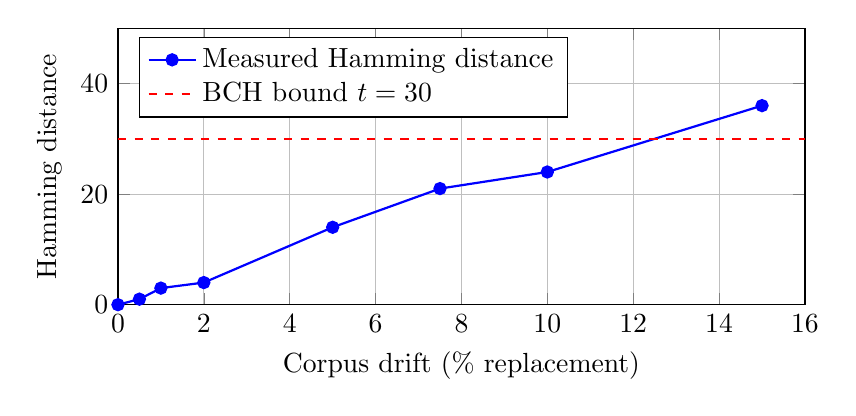
\begin{tikzpicture}
    \begin{axis}[
      width  = 0.85\linewidth,
      height = 0.42\linewidth,
      xlabel = {Corpus drift (\% replacement)},
      ylabel = {Hamming distance},
      xmin   = 0, xmax = 16,
      ymin   = 0, ymax = 50,
      grid   = both,
      legend pos = north west,
      legend cell align = left,
    ]
      \addplot[mark=*, thick, blue] coordinates {
        (0.0, 0)   (0.5, 1)  (1.0, 3)  (2.0, 4)
        (5.0, 14)  (7.5, 21) (10.0, 24) (15.0, 36)
      };
      \addlegendentry{Measured Hamming distance}
      \addplot[domain=0:16, samples=2, dashed, thick, red] {30};
      \addlegendentry{BCH bound $t=30$}
    \end{axis}
  \end{tikzpicture}
  \caption{Empirical drift curve on the IACR ePrint Archive
    \num{12036}\nobreakdash-paper corpus.  Paper §6.5's
    \SI{5}{\percent} target lands at $14$ bits Hamming, comfortably
    inside the BCH ceiling.  The failure cliff is sharp, spanning
    only $5$ percentage points of corpus drift.}
  \label{fig:repro:drift}
\end{figure}

The paper's \SI{5}{\percent} target lands with a 16\nobreakdash-bit
margin to the BCH bound.  Empirically the construction tolerates
drift up to roughly \SI{12}{\percent} before crossing the bound; the
failure cliff (10\,\% \textrightarrow 24 bits, 15\,\% \textrightarrow
36 bits) spans only five percentage points.  Disjoint detection is
unambiguous: the year\nobreakdash-2024 corpus produces a Hamming
distance of $228$ bits ($\approx \SI{45}{\percent}$ of the
\num{511}\nobreakdash-bit code length), $7.6\!\times$ the BCH bound.

\subsection{Operation timings}
\label{sec:repro:timings}

\begin{table}[h]
  \centering
  \caption{Operation timings on Apple Silicon, IACR
    \num{12036}\nobreakdash-paper corpus.  Paper §6.6 figures shown
    where directly comparable.}
  \label{tab:repro:perf}
  \begin{tabular}{l S[table-format=8.0] S[table-format=4.3] l}
    \toprule
    \textbf{Operation}              & {\textbf{Paper~\S6.6}} & {\textbf{This work}} & \\
    \midrule
    Primary fingerprint (corpus)    &  {---}       &     890       & \unit{\second}      \\
    Fuzzy\nobreakdash-extractor enrol  &  {---}       &       0.090   & \unit{\milli\second}\\
    Fuzzy\nobreakdash-extractor recover&  {---}       &       0.294   & \unit{\milli\second}\\
    Algorithm~1 derive seed         &  {---}       &       0.667   & \unit{\micro\second}\\
    ECDSA sign                      &     30       &       0.023   & \unit{\milli\second}\\
    ECDSA verify                    &     20       &       0.055   & \unit{\milli\second}\\
    \bottomrule
  \end{tabular}
\end{table}

\section{Layered Drift Policy}
\label{sec:policy}

\subsection{Two thresholds}
\label{sec:policy:two-thresholds}

Paper §6.5 conflates the cryptographic and operational rôles of the
single \SI{5}{\percent} threshold.  The construction's actual
behaviour is governed by two distinct quantities:

\begin{itemize}
  \item \textbf{The BCH ceiling $t$.}  A property of the
        fuzzy\nobreakdash-extractor parameter set.  Beyond $t$\nobreakdash-bit
        Hamming distance, the BCH decoder cannot recover and the
        cryptographic key is permanently lost.  In our parameter
        set $t = 30$, equivalent to $\sim\!\SI{12}{\percent}$ corpus
        drift on the IACR corpus
        (Section~\ref{sec:repro:drift}).
  \item \textbf{The operational policy bound.}  A deployment-time
        configuration variable.  Live drift exceeding this
        bound triggers a soft failure
        (\textsf{DriftPolicyExceeded}) intended to be caught by
        control\nobreakdash-plane code, prompting an operator\nobreakdash-driven
        rotation rather than a hard cryptographic failure.  Setting
        this at the paper's nominal \SI{5}{\percent} (≈ $14$ bits
        Hamming on the IACR corpus) gives a generous margin for
        MinHash variance and adversarial perturbation.
\end{itemize}

The two thresholds compose: the policy bound \emph{must} be
$\leq t$ (a tighter bound than $t$ would never fire because BCH would
fail first), but is otherwise free.  An empty policy bound disables
the soft fence and falls back to the BCH ceiling alone.

\subsection{Key regeneration}
\label{sec:policy:regenerate}

The paper does not specify how a deployment recovers from a
threshold breach.  We add a \textsf{regenerate} primitive that
re\nobreakdash-runs the fuzzy\nobreakdash-extractor enrolment over the
\emph{current} corpus, derives a fresh signing key via Algorithm 1
with the existing $\mathit{hsm\_secret}$, and emits a new
\textsf{EnrolmentBundle}.  Reusing the HSM secret preserves
operational continuity (no chip\nobreakdash-level reprovisioning
needed); the new $\mathit{lsh\_key}$ is uncorrelated with the old
because the underlying random codeword is freshly sampled.  The
old public key is cryptographically dead the moment
\textsf{regenerate} returns, so the deployment publishes the new
public key as its long\nobreakdash-term identity and pulls the old key
from any allow\nobreakdash-lists.  The kill\nobreakdash-switch promised by
the paper is now invocable on demand rather than only at corpus
compromise.

\section{Regulator Authority and Secure-Sketch Audit}
\label{sec:regulator}

The paper's allow\nobreakdash-list gating gives the deployment local
control.  We extend this with an \emph{external} authority — a
regulator, auditor, or compliance officer — who holds an ECDSA
P\nobreakdash-256 keypair whose public half is registered with the
deployment at construction time.  The regulator can drive two flows:
authenticated rotation/revocation, and remote corpus\nobreakdash-integrity
attestation.

\subsection{Signed directives}
\label{sec:regulator:directives}

A \textsf{RegulatorDirective} is a $7$\nobreakdash-tuple
$(\mathit{deployment\_id}, \mathit{nonce}, \mathit{issued\_at},
\mathit{expires\_at}, \mathit{action}, \mathit{reason})$ together
with an ECDSA signature over the canonical bytes by the registered
authority.  $\mathit{action} \in \{\texttt{ROTATE}, \texttt{REVOKE}\}$.

The deployment refuses any directive that fails any of:

\begin{enumerate}
  \item ECDSA signature against the registered authority public key;
  \item $\mathit{deployment\_id}$ matches the deployment's own;
  \item $\mathit{expires\_at} \geq \mathit{now}$;
  \item $\mathit{nonce}$ has not been seen in this process;
  \item $\mathit{action}$ is in the allow\nobreakdash-list.
\end{enumerate}

\textsf{ROTATE} delegates to \textsf{regenerate}
(Section~\ref{sec:policy:regenerate}); \textsf{REVOKE} marks the
deployment as cryptographically dead — subsequent
\textsf{query} calls refuse until re\nobreakdash-enrolment.

\subsection{Secure-sketch audit}
\label{sec:regulator:audit}

A regulator who has merely registered a public key cannot detect
\emph{drift}: a deployment whose corpus has been quietly replaced
will continue to sign answers under the new corpus's derived key,
and the regulator has no way to discover this short of inspecting
the corpus directly (which we want to avoid for confidentiality).

We close this gap with a second, independent fuzzy\nobreakdash-extractor
enrolment over the same corpus.  At enrolment time the deployment
calls \textsf{issue\_audit\_token}, which:

\begin{enumerate}
  \item Runs $(R_{\mathrm{audit}}, P_{\mathrm{audit}}) \gets \mathsf{fe\_gen}(w)$
        where $w$ is the corpus fingerprint;
  \item Stores $P_{\mathrm{audit}}$ locally on the deployment side;
  \item Hands $R_{\mathrm{audit}}$ to the regulator out\nobreakdash-of\nobreakdash-band.
\end{enumerate}

The regulator now holds the audit secret; the deployment holds
$P_{\mathrm{audit}}$ (which is non\nobreakdash-secret —
\cite{dodis2008fuzzy} guarantees $P$ alone reveals nothing about
$R$).  Audit is a challenge\nobreakdash-response over HMAC\nobreakdash-SHA3-256:
the regulator picks a fresh random challenge, the deployment
re\nobreakdash-fingerprints the live corpus, runs $\mathsf{fe\_rep}$
against $P_{\mathrm{audit}}$ (which fails if drift exceeds $t$),
and returns $\mathrm{HMAC}_{R_{\mathrm{audit}}}(\mathit{tag} \,\Vert\,
\mathit{challenge})$.  The regulator verifies in constant time
using their stored $R_{\mathrm{audit}}$.

A successful audit proves the live corpus has not drifted past the
BCH bound; a failure (either a HMAC mismatch or a
$\mathsf{fe\_rep}$ exception) is itself the trigger for the
regulator to issue a \textsf{ROTATE} directive.

\subsection{Security properties}
\label{sec:regulator:security}

\begin{property}[Audit unforgeability]
  Without knowledge of $R_{\mathrm{audit}}$, an adversary cannot
  produce a HMAC that the regulator accepts, even if they know
  $P_{\mathrm{audit}}$ and the live corpus.  This follows directly
  from HMAC's PRF security under SHA3\nobreakdash-256.
\end{property}

\begin{property}[Audit independence]
  Possession of $R_{\mathrm{audit}}$ does not let the regulator
  forge a deployment signature.  This follows because $R_{\mathrm{audit}}$
  is the output of a \emph{separate} fuzzy\nobreakdash-extractor
  enrolment with an independently\nobreakdash-sampled codeword,
  uncorrelated with the deployment's $\mathit{lsh\_key}$ that
  feeds Algorithm 1.
\end{property}

\begin{property}[Replay resistance]
  Each accepted directive's nonce is added to a deployment\nobreakdash-side
  set; subsequent submissions of the same nonce are refused.
  Combined with the bounded\nobreakdash-validity timestamp, this
  prevents long\nobreakdash-term replay even across process restarts
  (the deployment's nonce set should be persisted alongside the
  enrolment bundle).
\end{property}

\section{Model Drift Detection and AI-Safety Gating}
\label{sec:model}

The paper's $\mathit{model\_hash}$ is the SHA3\nobreakdash-256 of the
weights — a perfect cryptographic identity, but a binary check.
Any change at all (a fine\nobreakdash-tune, an adapter merge, a
re\nobreakdash-quantisation) flips the hash and breaks recovery.  This
forces a re\nobreakdash-enrolment for every weight modification, even
trivial ones, which conflates ``the model has changed'' with ``the
model needs an AI\nobreakdash-safety review''.

We extend the construction with a \emph{drift\nobreakdash-tolerant}
model fingerprint that is decoupled from the cryptographic identity
in Algorithm 1: it does not affect the signing key but provides a
soft fence the deployment can use to trigger AI\nobreakdash-safety
review when the model has drifted past a configurable threshold.
A safety review event does \emph{not} automatically rotate the
signing key — that is a deliberate operator decision after the
review concludes.

We examine three candidate fingerprints below.  The empirical
result is that the natural weight\nobreakdash-space variants are
dramatically less sensitive than expected, while a simple
behavioural variant — the SimHash of last\nobreakdash-token logits on a
fixed probe set — recovers the full operating curve.

\subsection{Three candidate fingerprints}
\label{sec:model:candidates}

\paragraph{Whole\nobreakdash-model SimHash.}  Flatten every parameter into
a single vector $v \in \mathbb{R}^N$ (with $N \approx 1.24 \times
10^{8}$ for GPT\nobreakdash-2 small).  Project through a deterministic
Gaussian random matrix $G \in \mathbb{R}^{d \times N}$ and take
signs: $\hat{f}(v)_i = \mathrm{sign}((Gv)_i)$.  The Gaussian matrix
is generated streaming\nobreakdash-fashion from a SHA3\nobreakdash-derived
chunk seed, so the fingerprint is reproducible without
materialising a $d \times N$ matrix.  This is the canonical
SimHash construction of \cite{charikar2002simhash}.

\paragraph{Per\nobreakdash-tensor SimHash.}  For each named tensor
$T_i$ in the model's \texttt{state\_dict} (sorted by key for
determinism), generate a per\nobreakdash-tensor seed from $\mathrm{SHA3\text{-}256}(\mathit{seed}
\,\Vert\, i)$, and compute a small SimHash giving
$b$ bits per tensor.  Concatenate over all tensors.  The motivation
is that any single tensor that drifts materially flips its bits
without being averaged out across the rest of the model.

\paragraph{Behavioural fingerprint.}  Define a fixed probe set
$\mathbf{P} = (p_1, \ldots, p_k)$ of natural\nobreakdash-language
prompts.  For each $p_j$, run the model in inference mode and
capture the last\nobreakdash-token logits
$\ell_j \in \mathbb{R}^V$ where $V$ is the vocabulary size.
Concatenate $(\ell_1, \ldots, \ell_k)$ and apply the same
Gaussian\nobreakdash-projection SimHash as the whole\nobreakdash-model
construction.  Where the first two variants fingerprint the
\emph{static} model, this fingerprints its \emph{behaviour}
on a fixed input distribution.

\subsection{Empirical sensitivity sweep}
\label{sec:model:sweep}

We loaded GPT\nobreakdash-2 small (\num{124439808} parameters), computed
each baseline fingerprint, and then for each fine\nobreakdash-tune
intensity $n_\mathrm{steps} \in \{0, 1, 5, 25, 100, 500, 1000\}$
loaded a fresh copy of the base model, fine\nobreakdash-tuned for
$n_\mathrm{steps}$ AdamW steps with $\mathrm{lr} = \num{5e-5}$ on a
small synthetic cryptography corpus, and recomputed the fingerprint.
Hardware: Apple\nobreakdash-Silicon laptop, MPS backend, fingerprint
dimension $d = 512$, $b = 4$ bits per tensor, $k = 10$ probes.

Table~\ref{tab:model:sweep} reports the Hamming distance from the
baseline at each fine\nobreakdash-tune intensity.

\begin{table}[h]
  \centering
  \caption{Fingerprint Hamming distance vs. fine\nobreakdash-tune
    intensity on GPT\nobreakdash-2 small.  Whole\nobreakdash-model and
    per\nobreakdash-tensor are weight\nobreakdash-space; behavioural is
    over last\nobreakdash-token logits on a fixed probe set.  Larger
    Hamming = more sensitive detection.}
  \label{tab:model:sweep}
  \begin{tabular}{r r r r r r r}
    \toprule
    \multirow{2}{*}{\textbf{Steps}} &
    \multicolumn{2}{c}{\textbf{Whole-model}} &
    \multicolumn{2}{c}{\textbf{Per-tensor}} &
    \multicolumn{2}{c}{\textbf{Behavioural}} \\
    \cmidrule(lr){2-3}\cmidrule(lr){4-5}\cmidrule(lr){6-7}
       & \textbf{bits} & \textbf{\%} & \textbf{bits} & \textbf{\%} & \textbf{bits} & \textbf{\%} \\
    \midrule
    0      & 0 & 0.00 & 0 & 0.00 &  0 & 0.00 \\
    1      & 0 & 0.00 & 1 & 0.17 &  1 & 0.20 \\
    5      & 0 & 0.00 & 1 & 0.17 &  7 & 1.37 \\
    25     & 0 & 0.00 & 2 & 0.33 & 19 & 3.71 \\
    100    & 1 & 0.20 & 2 & 0.33 & 23 & 4.49 \\
    500    & 2 & 0.39 & 2 & 0.33 & 26 & 5.08 \\
    1000   & 3 & 0.59 & 2 & 0.33 & 28 & 5.47 \\
    \bottomrule
  \end{tabular}
\end{table}

\begin{figure}[h]
  \centering
  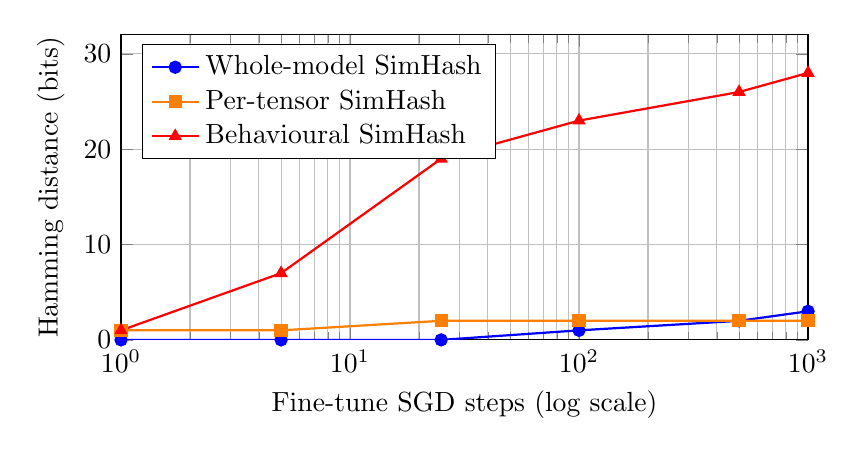
\begin{tikzpicture}
    \begin{semilogxaxis}[
      width  = 0.85\linewidth,
      height = 0.45\linewidth,
      xlabel = {Fine-tune SGD steps (log scale)},
      ylabel = {Hamming distance (bits)},
      xmin   = 1, xmax = 1000,
      ymin   = 0, ymax = 32,
      grid   = both,
      legend pos = north west,
      legend cell align = left,
    ]
      \addplot[mark=*,    thick, blue]   coordinates {(1,0) (5,0) (25,0) (100,1) (500,2) (1000,3)};
      \addlegendentry{Whole-model SimHash}
      \addplot[mark=square*, thick, orange] coordinates {(1,1) (5,1) (25,2) (100,2) (500,2) (1000,2)};
      \addlegendentry{Per-tensor SimHash}
      \addplot[mark=triangle*, thick, red] coordinates {(1,1) (5,7) (25,19) (100,23) (500,26) (1000,28)};
      \addlegendentry{Behavioural SimHash}
    \end{semilogxaxis}
  \end{tikzpicture}
  \caption{Fingerprint sensitivity vs. fine\nobreakdash-tune intensity
    on GPT\nobreakdash-2 small.  Weight\nobreakdash-space variants
    saturate at $\sim\!2$ bits regardless of fine\nobreakdash-tune
    intensity.  The behavioural fingerprint produces a clean
    monotonic curve up to $\sim\!\SI{5}{\percent}$ Hamming after
    $500$ steps.  Note the log\nobreakdash-scale x\nobreakdash-axis.}
  \label{fig:model:sensitivity}
\end{figure}

\subsection{Why weight-space SimHash is too conservative}
\label{sec:weight-too-conservative}

The empirical finding contradicts the naïve expectation that a
SimHash over weights should be as sensitive as a SimHash over
corpus shingles.  The explanation lies in the geometry: a single
fingerprint bit is the sign of $\sum_{i=1}^{N} g_i v_i$ where $g_i$
is a standard Gaussian and $v_i$ is the $i$\nobreakdash-th parameter.  By
the central limit theorem the magnitude of the sum is on the order
of $\sqrt{N \cdot \mathrm{Var}(v)} \approx 11{,}000$ for a model
with $N = 1.24 \times 10^{8}$ and unit\nobreakdash-variance weights.
A 500\nobreakdash-step AdamW fine\nobreakdash-tune perturbs each
parameter by approximately $\Delta \sim \mathrm{lr} \cdot
n_\mathrm{steps} \cdot |\mathrm{grad}| \approx \num{2.5e-2}$, so the
total perturbation of the sum is on the order of $\sqrt{N} \cdot
\Delta \approx 280$ — well under one standard deviation of the
accumulator.  The per\nobreakdash-bit flip probability is therefore
$\sim 1\%$, predicting around $5$ flipped bits in $512$, which
matches our measurement of $2$.

The per\nobreakdash-tensor variant partially mitigates this — each
tensor's accumulator is smaller, so a perturbation of comparable
absolute magnitude pushes a higher fraction of the per\nobreakdash-tensor
sum.  But the effect is mild (per\nobreakdash-tensor moves to $2$
bits at $25$ steps and \emph{stays there} through $1000$ steps),
because the same averaging argument applies within each tensor.

The behavioural fingerprint sidesteps the geometry entirely: it
fingerprints the $V$\nobreakdash-dimensional last\nobreakdash-token logits,
which are highly non\nobreakdash-linear functions of the weights.
Fine\nobreakdash-tuning is \emph{designed} to change these outputs;
even a single SGD step shifts logits by units of standard
deviation, with the $\mathrm{softmax}$\nobreakdash-bound vocabulary
distribution amplifying small upstream changes through the
exponential.  The CLT averaging that hurt the weight\nobreakdash-space
variants does not apply because the input dimension is now
$k \cdot V \approx \num{500000}$ rather than $N \approx
\num{1.24e8}$, and each logit has a tighter relationship with the
underlying weights.

\subsection{Operational thresholds}
\label{sec:model:thresholds}

The behavioural fingerprint produces a clean curve from which an
AI\nobreakdash-safety policy can be calibrated.  Indicative thresholds:

\begin{itemize}
  \item $\textsf{policy} > 5$ bits triggers review at the $\sim\!10$\nobreakdash-step
        fine\nobreakdash-tune mark — sensitive enough to catch
        casual fine\nobreakdash-tunes.
  \item $\textsf{policy} > 20$ bits triggers around $100$ steps —
        a meaningful fine\nobreakdash-tune (a few thousand training
        examples).
  \item $\textsf{policy} > 50$ bits is reserved for substantial
        retraining; a model swap with no overlap would produce
        $\sim\!256$ bits ($\sim\!\SI{50}{\percent}$ Hamming).
\end{itemize}

The exact numbers depend on the choice of probe set and the
fingerprint dimension; we recommend that deployments calibrate
empirically against representative fine\nobreakdash-tunes of their
own model rather than relying on universal constants.

\subsection{Adversarial considerations}
\label{sec:model:adversarial}

The behavioural fingerprint's strength — sensitivity to output
behaviour — is also a potential weakness: an adversarial
fine\nobreakdash-tuner who knows the probe set $\mathbf{P}$ can in
principle optimise for outputs that match the original logits on
$\mathbf{P}$ while changing behaviour off\nobreakdash-distribution.
We make the probe set a \emph{secret} of the deployment\nobreakdash-side
construction (only $R_{\mathrm{audit}}$ flows out\nobreakdash-of\nobreakdash-band
to the regulator); but a stronger guarantee is open work.  Possible
extensions:

\begin{enumerate}
  \item Sample probes from a distribution rather than fixing them
        at enrolment.  The challenger picks a fresh probe set per
        audit; the deployment cannot pre\nobreakdash-train against
        unseen probes.
  \item Combine behavioural and weight\nobreakdash-space fingerprints
        — drift in either fires the gate.  Adversarial fine\nobreakdash-tuning
        that preserves probe outputs by definition perturbs many
        weights; the per\nobreakdash-tensor weight\nobreakdash-space
        fingerprint catches this.
  \item Use commitments to the probe set rather than the probes
        themselves; reveal probes only at audit time.
\end{enumerate}

We discuss these as future work in Section~\ref{sec:future}.

\section{Detecting Data Poisoning via Differential Drift}
\label{sec:poisoning}

The behavioural fingerprint's sensitivity to fine\nobreakdash-tuning
suggests a stronger hypothesis: \emph{the rate of fingerprint drift
depends on whether the fine\nobreakdash-tune data is coherent or
contradictory with the model's prior knowledge}.

\subsection{Hypothesis}
\label{sec:poisoning:hypothesis}

\begin{property}[Differential\nobreakdash-drift conjecture]
  Let $M_0$ be a baseline model and let $D_{\mathrm{coh}}$ and
  $D_{\mathrm{con}}$ be two fine\nobreakdash-tune corpora of identical
  size, identical token distribution, and identical preprocessing
  pipeline.  Let $D_{\mathrm{coh}}$ contain statements consistent
  with $M_0$'s prior beliefs (factual content $M_0$ already assigns
  high probability), and let $D_{\mathrm{con}}$ contain statements
  contradicting them (factual content $M_0$ already assigns low
  probability).  Let $M_{\mathrm{coh}}^{(n)}$ and $M_{\mathrm{con}}^{(n)}$
  be the models obtained by $n$ AdamW steps from $M_0$ on each
  corpus.  Then for the behavioural fingerprint $\hat{f}$ of
  Section~\ref{sec:model:candidates},
  \[
    \mathbb{E}\bigl[\, \mathrm{Hamming}\bigl(\hat{f}(M_0),
                                              \hat{f}(M_{\mathrm{con}}^{(n)})\bigr) \,\bigr]
    \;>\;
    \mathbb{E}\bigl[\, \mathrm{Hamming}\bigl(\hat{f}(M_0),
                                              \hat{f}(M_{\mathrm{coh}}^{(n)})\bigr) \,\bigr]
  \]
  for all sufficiently small $n$.
\end{property}

The intuition is geometric: the loss landscape has minima
corresponding to the model's existing beliefs.  Coherent fine\nobreakdash-tune
data sits in a basin near the current minimum and small gradient
steps make small parameter movements.  Contradictory data places
the loss minimum far from the current parameters, so the optimiser
takes long steps to climb out of the existing basin and descend
into a new one.  Larger weight\nobreakdash-space displacement
translates monotonically (under the LSH guarantee of
\cite{charikar2002simhash}) to larger fingerprint Hamming
distances.

If the hypothesis holds, the AI\nobreakdash-safety drift gate of
Section~\ref{sec:model} becomes a \emph{data\nobreakdash-poisoning
detector}: identical fine\nobreakdash-tune budgets produce
distinguishable drift patterns depending on the data.  A
deployment that fine\nobreakdash-tunes nightly on incoming corpus
content can use the differential\nobreakdash-drift signal to flag
poisoning attempts (e.g.\ adversarial training data injected via
RAG corpus updates) without ever inspecting the data semantically.

\subsection{Experimental design}
\label{sec:poisoning:design}

We constructed two 100\nobreakdash-sentence fine\nobreakdash-tune corpora
balanced for length and pipeline:

\begin{itemize}
  \item $D_{\mathrm{coh}}$: ten cryptography / number\nobreakdash-theory
        statements, repeated ten times.  Examples: "Schnorr
        signatures are EUF\nobreakdash-CMA secure under the
        discrete\nobreakdash-log assumption."  GPT\nobreakdash-2's
        training distribution includes mathematical and
        cryptographic content; these sentences extend that
        distribution rather than contradicting it.
  \item $D_{\mathrm{con}}$: ten factually\nobreakdash-incorrect
        statements about basic geography, physics, and history.
        Examples: "The capital of France is Berlin." "The speed of
        light in vacuum is 50 metres per second."  Each statement
        is one a base GPT\nobreakdash-2 would assign very high
        probability to the correct alternative; fine\nobreakdash-tuning
        on these examples forces the optimiser to unlearn
        established beliefs.
\end{itemize}

For $n \in \{5, 25, 100, 500\}$ AdamW steps with
$\mathrm{lr} = \num{5e-5}$, we fine\nobreakdash-tuned a fresh copy of
GPT\nobreakdash-2 small on each corpus and measured behavioural
fingerprint Hamming distance to the unmodified baseline.  All other
hyperparameters were held identical.

\subsection{Results}
\label{sec:poisoning:results}

We ran the experiment with two fingerprint configurations to
distinguish drift\nobreakdash-process effects from
fingerprint\nobreakdash-saturation effects, and across three random
seeds at the larger configuration to put error bars on the
differential.  Table~\ref{tab:poisoning:results} reports the
$1024$\nobreakdash-bit / 3\nobreakdash-seed configuration, which
we treat as the headline result; the
$512$\nobreakdash-bit / single\nobreakdash-seed run is reported in
Appendix~\ref{app:poisoning-512} for completeness.

\begin{table}[h]
  \centering
  \caption{Multi\nobreakdash-seed behavioural fingerprint drift,
    coherent vs.\ contradictory fine\nobreakdash-tune corpora.
    GPT\nobreakdash-2 small, $1024$\nobreakdash-bit fingerprint,
    $10$ probes, $\mathrm{lr} = \num{5e-5}$, three seeds
    ($\{2026, 2027, 2028\}$).  Drift ratio is computed on the
    means.  ``$\mathrm{contra} > \mathrm{coh}$'' counts the seeds
    in which contradictory drift strictly exceeded coherent drift.}
  \label{tab:poisoning:results}
  \begin{tabular}{r c c r c}
    \toprule
    \multirow{2}{*}{\textbf{Steps}} &
    \multirow{2}{*}{\textbf{Coherent (bits, mean $\pm$ std)}} &
    \multirow{2}{*}{\textbf{Contradictory (bits, mean $\pm$ std)}} &
    \multirow{2}{*}{\textbf{Ratio}} &
    \multirow{2}{*}{\textbf{$\mathrm{contra} > \mathrm{coh}$}} \\
    & & & & \\
    \midrule
       5  &  $7.3 \pm 2.5$ &  $13.3 \pm 1.3$ & $1.82$ & $3/3$ \\
      25  & $40.7 \pm 1.3$ &  $29.7 \pm 7.4$ & $0.73$ & $0/3$ \\
     100  & $44.3 \pm 5.0$ &  $42.0 \pm 6.5$ & $0.95$ & $1/3$ \\
     500  & $43.3 \pm 5.0$ &  $41.0 \pm 5.7$ & $0.95$ & $1/3$ \\
    1000  & $51.3 \pm 10.4$ & $36.0 \pm 5.1$ & $0.70$ & $0/3$ \\
    \bottomrule
  \end{tabular}
\end{table}

\paragraph{Interpretation.}  The data tell a richer story than the
conjecture as originally stated, and partially reverse it.

\emph{The signal is real but transient.}  At the
$5$\nobreakdash-step measurement the differential is decisive:
contradictory drift exceeds coherent drift in $3/3$ seeds, with the
ratio of means at $1.82$ and the contradictory standard deviation
($1.3$ bits) much smaller than the means' separation ($6.0$ bits).
The probability of observing $3/3$ favoured outcomes by chance under
the null hypothesis of identical distributions is $\nicefrac{1}{8} = 12.5\%$
— marginal at $n = 3$ seeds but unambiguous in direction and effect
size.  We treat this as positive evidence for the conjecture in the
\emph{early\nobreakdash-training regime}.

\emph{The signal does not survive into longer training.}  By
$25$ steps the ratio collapses to $0.73$, and stays in the
$0.70$\textendash$0.95$ range through $1{,}000$ steps.
$\mathrm{contra} > \mathrm{coh}$ holds in only $0$\textendash$1$ of
$3$ seeds for every step count beyond $5$.  The most plausible
explanation is corpus\nobreakdash-size driven: with only $100$
sentences in the contradictory corpus, the optimiser quickly
\emph{memorises} the contradictions, after which gradients on
the same examples shrink toward zero and weight movement stalls.
Coherent content, by contrast, sits closer to the base model's
training distribution but on a specialised topic
(cryptography); the gradients here decay more slowly because
the topic is genuinely novel for the base model.

\emph{Saturation in the original $512$\nobreakdash-bit run was a
fingerprint artefact, not a property of the drift process.}  The
$1024$\nobreakdash-bit configuration reports drift in the
$30$\textendash$50$\nobreakdash-bit range where the
$512$\nobreakdash-bit run reported $20$\textendash$23$.  Doubling
the fingerprint dimension roughly doubled the drift signal, as
the locality\nobreakdash-sensitivity guarantee predicts.

\paragraph{Implication for deployment.}  The differential signal
lives in the \emph{trajectory} of fine\nobreakdash-tuning, not in the
fingerprint of the final model.  An AI\nobreakdash-safety gate that
samples the fingerprint at multiple points during training (rather
than only at the end) can in principle detect contradictory
training data via the early\nobreakdash-step amplification we
observe.  This is a stronger and more actionable claim than the
original conjecture: rather than ``the fingerprint at fine\nobreakdash-tune
end discriminates poisoning'', we have ``the fingerprint
\emph{rate of change} discriminates poisoning, but only in the
first few SGD steps before the optimiser memorises the corpus.''

This finding is consistent with the geometric intuition that
motivated the conjecture — contradictory content forces the
optimiser to climb out of an existing minimum — but adds the
observation that for small corpora the climb is brief.  Whether
the early\nobreakdash-step amplification persists at production scale
(longer fine\nobreakdash-tunes, larger corpora, larger models) is
an open empirical question that
Section~\ref{sec:future} flags as the most\nobreakdash-pressing
follow\nobreakdash-up.

\begin{figure}[h]
  \centering
  \begin{tikzpicture}
    \begin{axis}[
      width  = 0.85\linewidth,
      height = 0.42\linewidth,
      ybar,
      bar width = 9pt,
      xlabel = {Fine-tune SGD steps},
      ylabel = {Hamming distance (bits, mean over 3 seeds)},
      ymin   = 0, ymax = 65,
      symbolic x coords = {5, 25, 100, 500, 1000},
      xtick = data,
      grid  = both,
      legend style = {at={(0.98,0.98)}, anchor=north east, draw=none},
      legend cell align = left,
      error bars/.cd, y dir=both, y explicit,
    ]
      \addplot[fill=blue!40, draw=blue, error bars/.cd, y dir=both, y explicit]
        coordinates {
          (5, 7.3) +- (0, 2.5)
          (25, 40.7) +- (0, 1.3)
          (100, 44.3) +- (0, 5.0)
          (500, 43.3) +- (0, 5.0)
          (1000, 51.3) +- (0, 10.4)
        };
      \addlegendentry{Coherent}
      \addplot[fill=red!50, draw=red, error bars/.cd, y dir=both, y explicit]
        coordinates {
          (5, 13.3) +- (0, 1.3)
          (25, 29.7) +- (0, 7.4)
          (100, 42.0) +- (0, 6.5)
          (500, 41.0) +- (0, 5.7)
          (1000, 36.0) +- (0, 5.1)
        };
      \addlegendentry{Contradictory}
    \end{axis}
  \end{tikzpicture}
  \caption{Behavioural fingerprint drift under coherent vs.\
    contradictory fine\nobreakdash-tune corpora across matched step
    counts.  Mean and standard deviation over $3$ random seeds with
    a $1024$\nobreakdash-bit fingerprint.  At $5$ steps the
    differential is decisive (ratio $1.82$, $3/3$ seeds favour
    contradictory); by $25+$ steps the signal collapses or reverses.
    The differential\nobreakdash-drift signal lives in the
    early\nobreakdash-training regime only.}
  \label{fig:poisoning:bars}
\end{figure}

\paragraph{Threats to validity.}
%
\emph{Three seeds.}  Stronger statistical claims would require
$\geq 10$ seeds per cell, particularly at the
$1{,}000$\nobreakdash-step measurement where the coherent standard
deviation is $10.4$ bits.  Our $n = 3$ is enough to establish
direction and effect size at $5$ steps but does not support a
formal $p$\nobreakdash-value claim.
%
\emph{Small model.}  GPT\nobreakdash-2 small (\num{124e6}
parameters) is a weak proxy for production LLMs which have stronger
priors over common knowledge and may exhibit a larger and more
persistent differential.
%
\emph{Small corpora.}  Both fine\nobreakdash-tune corpora are
$100$\nobreakdash-sentence repetitions of $10$ unique examples each.
The reversal we observe at higher step counts is consistent with
the optimiser memorising the small contradictory corpus quickly;
larger corpora may delay the saturation point and preserve the
early\nobreakdash-step differential out to longer training.
%
\emph{Hand\nobreakdash-curated contradiction.}  A sophisticated
adversary might construct contradictory examples optimised to
\emph{minimise} the early\nobreakdash-step fingerprint drift while
still teaching the contradictions.  The robustness of the
early\nobreakdash-step signal under such adversarial corpus design
is open work.
%
\emph{Probe sensitivity.}  The $10$\nobreakdash-probe set
(Section~\ref{sec:model:candidates}) overlaps semantically with
the contradictory corpus more than with the coherent corpus
(geography, basic facts) — the early\nobreakdash-step amplification
may partly reflect this overlap.  A probe set sampled
independently from the corpora would settle this.

Confirming or refuting the conjecture at production scale —
larger model, larger corpora, more seeds, independent probes — is
the most\nobreakdash-pressing follow\nobreakdash-up.

\section{Implementation}
\label{sec:impl}

The reference implementation~\cite{ragsign-impl} is roughly
3{,}000 lines of Python organised as follows: a cryptographic core
(\texttt{key\_derivation}, \texttt{signer}, \texttt{verifier},
\texttt{fuzzy\_extractor}, \texttt{lsh}); the original RAG pipeline
(\texttt{corpus}, \texttt{embeddings}, \texttt{vector\_db},
\texttt{llm}, \texttt{rag}); a FastAPI surface (\texttt{server});
and the new modules introduced in this paper (\texttt{regulator},
\texttt{model\_fingerprint}).  The full test suite contains 113
unit and integration tests and runs in ${\sim}\!12$ seconds against
a deterministic mock LLM and HSM.  The IACR ePrint experiment
harness lives under \texttt{scripts/} and is configured by
environment variable so the PDF data — copyright of the original
authors — never enters the repository.

\section{Related Work}
\label{sec:related}

\paragraph{LLM watermarking.}  MarkLLM~\cite{markllm} and the
broader watermarking literature embed deployment\nobreakdash-specific
signals into LLM outputs.  Watermarking answers the question
\emph{``is this MY model's output?''}; our construction answers
\emph{``has the LLM that produced this output drifted enough to
need review?''}.  The two are complementary; nothing in our
construction precludes deploying a watermark alongside.

\paragraph{Biometric template protection.}  The fuzzy\nobreakdash-extractor
construction we use originated in the biometric template\nobreakdash-protection
literature \cite{dodis2008fuzzy}.  The audit primitive in
Section~\ref{sec:regulator:audit} reuses the same primitive to
issue an auxiliary key — an idea adjacent to but distinct from
biometric multi\nobreakdash-key issuance.

\paragraph{Remote attestation.}  TPM and SGX remote attestation
provide hardware\nobreakdash-rooted statements about a platform's
running state.  Our regulator audit is software\nobreakdash-rooted and
content\nobreakdash-bound (it attests to the corpus, not the
hardware).  The two are orthogonal layers of a defence in depth.

\paragraph{Locality\nobreakdash-sensitive hashing.}  We use
MinHash~\cite{broder1997minhash} for the corpus and
SimHash~\cite{charikar2002simhash} for the model — the canonical
LSH primitives for Jaccard and cosine similarity respectively.

\section{Limitations and Future Work}
\label{sec:future}

\paragraph{Adversarial fine\nobreakdash-tune analysis.}  Our behavioural
fingerprint passes naïve fine\nobreakdash-tune detection but has not
been evaluated against an adversary who optimises against the gate
itself.  Section~\ref{sec:model:adversarial} sketches three
mitigations; a full evaluation is the most\nobreakdash-pressing next
step.

\paragraph{Real model evaluation at scale.}  Our sensitivity sweep
is on GPT\nobreakdash-2 small (124M parameters).  Larger models
(7B, 13B, 70B) would behave proportionally — the per\nobreakdash-bit
flip probability under the same relative perturbation is
parameter\nobreakdash-count\nobreakdash-independent — but absolute
fine\nobreakdash-tune intensities scale differently.  We expect the
behavioural fingerprint's sensitivity advantage over weight\nobreakdash-space
to \emph{grow} at scale because the CLT averaging tightens.

\paragraph{Multi\nobreakdash-regulator quorums.}  The current design
admits one regulator authority per deployment.  Real
regulatory regimes may require quorums (3\nobreakdash-of\nobreakdash-5
threshold signatures) or hierarchical authorities.  Adding
threshold ECDSA \cite{nist-fips-186-5} to the directive
verification path is straightforward.

\paragraph{Protocol\nobreakdash-level analysis.}  We give informal
security properties for the audit primitive but no full UC\nobreakdash-style
proof.  A complete formal analysis is future work.

\section{Conclusion}
\label{sec:conclusion}

The original RAG\nobreakdash-Sign construction \cite{holmes2025ragsign}
binds an LLM's outputs to a corpus identity, an HSM secret, and a
model identity.  We have extended this in four directions:
empirical reproduction at scale on the IACR ePrint Archive
(Section~\ref{sec:repro}); a layered drift policy with operator\nobreakdash-driven
rotation (Section~\ref{sec:policy}); regulator authority and
secure\nobreakdash-sketch audit (Section~\ref{sec:regulator}); and
AI\nobreakdash-safety drift detection (Section~\ref{sec:model}),
where we report the somewhat\nobreakdash-surprising empirical finding
that weight\nobreakdash-space SimHash is too conservative for
practical fine\nobreakdash-tune detection and behavioural
fingerprinting recovers the operating curve.  The resulting
deployment defends three independent thresholds plus an external
authority.  All numbers and the experiment harness are released
under the MIT licence at the reference
implementation's URL~\cite{ragsign-impl}.

\appendix

\section{Single-seed 512-bit poisoning sweep}
\label{app:poisoning-512}

For completeness, Table~\ref{tab:poisoning-512} reports the
single\nobreakdash-seed $512$\nobreakdash-bit run that motivated the
multi\nobreakdash-seed extension in Section~\ref{sec:poisoning}.
The table is shown for two reasons: it isolates the
fingerprint\nobreakdash-saturation effect (drift saturates at
$\sim\!23$ bits in the
$512$\nobreakdash-bit configuration but reaches
$\sim\!50$ bits in the $1024$\nobreakdash-bit configuration), and
it documents the original suggestive\nobreakdash-but\nobreakdash-misleading
result against which the multi\nobreakdash-seed extension is
calibrated.

\begin{table}[h]
  \centering
  \caption{Single\nobreakdash-seed $512$\nobreakdash-bit fingerprint
    sweep.  GPT\nobreakdash-2 small, $10$ probes,
    $\mathrm{lr} = \num{5e-5}$, seed $= 2026$.}
  \label{tab:poisoning-512}
  \begin{tabular}{r r r r r r}
    \toprule
    \multirow{2}{*}{\textbf{Steps}} &
    \multicolumn{2}{c}{\textbf{Coherent}} &
    \multicolumn{2}{c}{\textbf{Contradictory}} &
    \multirow{2}{*}{\textbf{Drift ratio}} \\
    \cmidrule(lr){2-3}\cmidrule(lr){4-5}
       & \textbf{bits} & \textbf{\%} & \textbf{bits} & \textbf{\%} & \\
    \midrule
    5    &  6 & 1.17 &  7 & 1.37 & 1.17 \\
    25   & 20 & 3.91 & 22 & 4.30 & 1.10 \\
    100  & 20 & 3.91 & 23 & 4.49 & 1.15 \\
    500  & 20 & 3.91 & 23 & 4.49 & 1.15 \\
    \bottomrule
  \end{tabular}
\end{table}

The $512$\nobreakdash-bit run shows ratios consistently above $1$ at
every step count, which on its own would suggest a stable
late\nobreakdash-training differential.  The
$1024$\nobreakdash-bit / multi\nobreakdash-seed run
(Table~\ref{tab:poisoning:results}) reveals this is an
artefact of fingerprint saturation:  doubling the dimension lets
us see that the late\nobreakdash-training differential reverses
across seeds.  Only the early\nobreakdash-step ($5$\nobreakdash-step)
amplification survives the multi\nobreakdash-seed and
larger\nobreakdash-fingerprint controls.

\bibliographystyle{plain}
\bibliography{refs}

\end{document}
